\subsection{Painting}
\label{sec:painting-cars}



In this section we consider spray painting objects with a robotic arm.
The goals are to cover the entire surface with a uniform amount
of paint, minimize the time the process takes, and minimize waste.

One strategy is to pick a start curve, then construct subsequent passes 
by shifting every point of the given curve a fixed distance along the
normal direction. Such a curve is called an \emph{offset curve} curve and
a offset curve planner constructs a coverage path from a given
start curve using the same spacing between adjacent passes.
See \figref{car-door}
for an example of painting a car door.


\begin{figure}[htb]
        \centering
        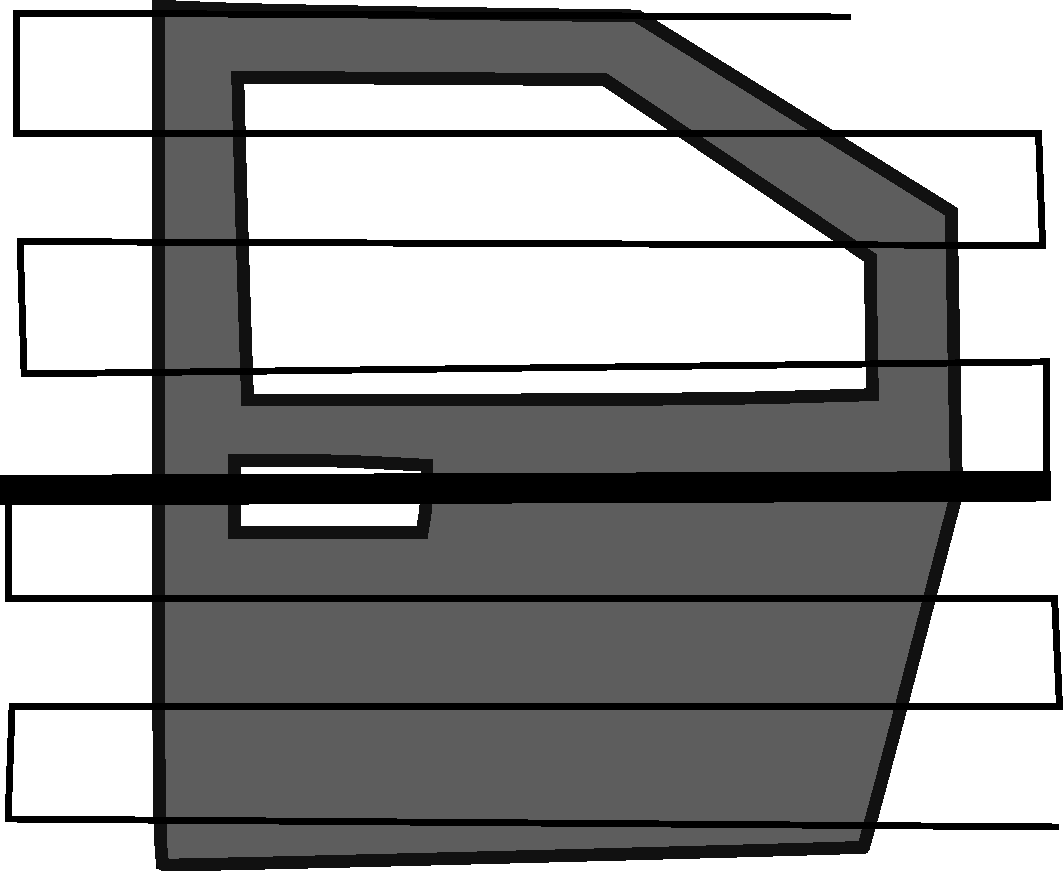
\includegraphics[width=.25\textwidth]{car-door-1}
		\caption{An example of a path traced when painting a car door.
		The start curve is bolded.
		\label{fig:car-door}}
\end{figure}

But how do we pick a start curve that meets our objectives of uniform paint coverage 
and minimal time?
In \cite{atkar_towards_2003,atkar_uniform_2005}, the authors
use the Gauss-Bonnet theorem to characterize start curves that 
meet our objects. 
More specifically, the Gauss-Bonnet theorem is used to  select the geodesic
start curve that minimizes the geodesic curvature of the
subsequent offset curves. 

Let $C_{st}$  be a segment of a smooth start curve $\gamma_0$
with end points $\gamma_0(t_0)$ and $\gamma_0(t_1)$ and let
$C_{of}$ be the offset curve of $C_{st}$ of $\gamma_\nabla$
with end points $\gamma_\Delta(t_0)$ and $\gamma_\Delta(t_1).$
The goal is to compute the integral of the geodesic curvature along $C_{of}.$
Define the quadrilateral in fig 6.

We apply the Gauss-Bonnet theorem to the regions $\phi_1$ and $\phi_2$ to
obtain
\begin{equation}\label{eqn:phi-1}
\int_{\phi_1}K+\int_{\partial\phi_1}k_g=(\theta_1+\theta_2+\theta_3)-\pi,
\end{equation}
\begin{equation}\label{eqn:phi-2}
\int_{\phi_2}K+\int_{\partial\phi_2}k_g=(\theta_4+\theta_5+\theta_6)-\pi,
\end{equation}

The curve $\gamma_{t_0}$ and $\gamma_{t_1}$ are geodesics
their geodesic curvature is zero and
\begin{equation}\label{eqn:phi-sum}
\int_{\partial\phi_1}k_g+\int_{\partial\phi_2}k_g=\int_{C_{st}}k_g -\int_{C_{of}}k_g
\end{equation}
and it follows that 
\begin{equation}\label{eqn:phi-sum}
\int_{\phi}K+\int_{C_{st}}k_g -\int_{C_{of}}k_g=(\theta_1+\theta_6)+\theta_2 +(\theta_3+\theta_4)+\theta_5-2\pi.
\end{equation}

...then the maximum between $\int_{C_\ell} k_g$ and $\int_{C_h} k_g$ is minimized when
$\int_{\phi^-}K=\int_{\phi^+}K$ and the integral of the geodesic curvature on the offset path
is minimized when the start curve $\gamma$ splits the surface into two disjoint regions
such that $\int_{\phi^-}K=\int_{\phi^+}K=\frac{1}{2}\int_S K$ a curve with this property
is called a \emph{Gaussian curvature divider}.

'Therefore, for practical implementation, we determine the start curve as a planar intersection curve that
is also a Gaussian curvature divider. There are multiple
planar intersection curves which are Gaussian curvature
dividers; we will select one that minimizes the cycle time.'